\documentclass[journal,12pt,twocolumn]{IEEEtran}
\usepackage{amsmath,amssymb,amsfonts,amsthm}
\usepackage{txfonts}
\usepackage{tkz-euclide}
\usepackage{listings}
\usepackage{gvv}
\usepackage[latin1]{inputenc}
\usepackage{array}
\usepackage{pgf}
\usepackage{lmodern}

\begin{document}
\bibliographystyle{IEEEtran}

\vspace{3cm}

\title{}
\author{EE23BTECH11054 -  Sai Krishna Shanigarapu$^{*}$
}
\maketitle
\newpage
\bigskip

% \renewcommand{\thefigure}{\theenumi}
% \renewcommand{\thetable}{\theenumi}

\section*{Exercise 9.2}

\noindent \textbf{13} \hspace{2pt}If the sum of $n$ terms of an A.P. is $3n^2+5n$ and its $m^{th}$ term is 164, find the value of $m$ and obtain the Z-transform of the series.
\bigskip

\noindent Solution:
\noindent
\begin{align}
S(n) &= 3\brak{n+1}^2 + 5\brak{n+1}\\
x\brak{n} &= \brak{x\brak{0} + nd}\brak{u\brak{n}}
\end{align}

\begin{align}
   S_0 &= 8\\
   S_1 &=22\\
    d &= 6\\
    m &= 26\\
    x \brak{n} &= \brak{8 + 6n} \brak{u\brak{n}} \label{x(n)}
\end{align}

\begin{figure}[h]
    \centering
    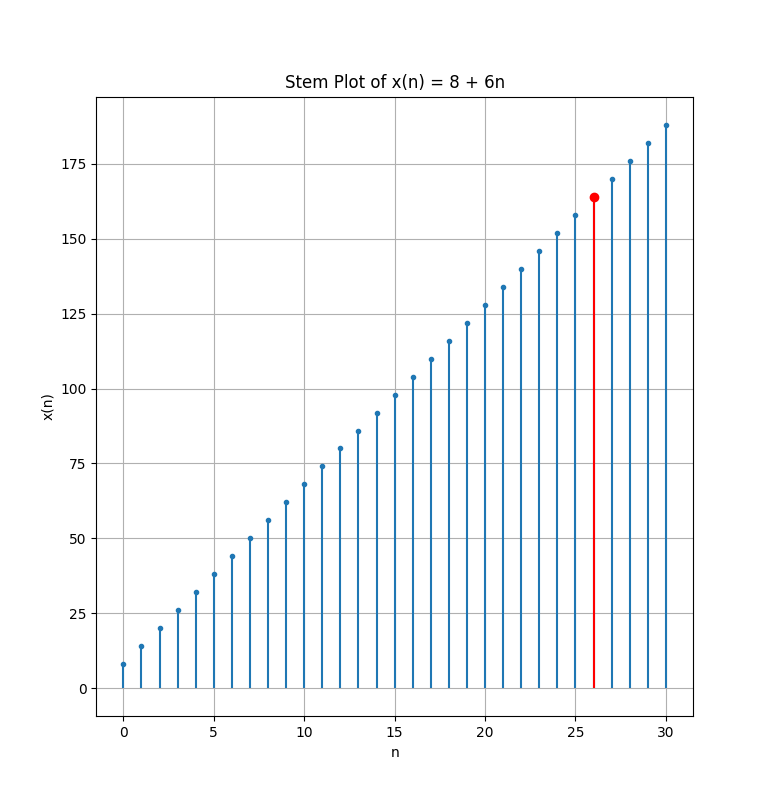
\includegraphics[width=1\columnwidth]{figs/Figure_1.png}
    \caption{Plot of x(n) vs n}
    \label{fig:11.9.2.13.1}
\end{figure}

\begin{align}
     x \brak{n} \system{Z} X \brak{z} 
\end{align}

\begin{align}
     X \brak{z} & = \sum_{n=-\infty}^{\infty} x \brak{n}  z^{-n}\\
     & = \sum_{n=0}^{\infty} \brak{8 + 6n} z^{-n} & \text{using } \eqref{x(n)}\\
     & = \frac{8-2z^{-1}}{\brak{1-z^{-1}}^2} & \cbrak{z\in\mathbb{C} : |z^{-1}| < 1}
\end{align}

So, the Z-transform of the given series is 
$$X\brak{z} = \frac{8-2z^{-1}}{\brak{1-z^{-1}}^2}$$

\setlength{\arrayrulewidth}{0.3mm}
\setlength{\tabcolsep}{15pt}
\renewcommand{\arraystretch}{1.4}

\begin{table}[ht]
\centering

\begin{tabular}{|c|c|}
\hline

\textbf{Symbol} & \textbf{Remarks}\\
\hline
$y\brak{n} =\brak{3n^2+11n+8}\brak{u\brak{n}}$ & Sum of $n$ terms  \\
\hline
$x(m-1)$ & $164$\\
\hline
$y\brak{n}$ & $x\brak{n} * u\brak{n}$\\
\hline
$Z_{z}^{-1}\brak{1-z^{-1}}^{-2}$ & $u\brak{n}$\\
\hline

\end{tabular}
\vspace{0.25cm}
\caption{Parameters}
%\label{tab:11.9.2.13.1}



\end{table}


\end{document}